\documentclass[a4paper,11pt,twoside]{article}
\usepackage[top=3cm,bottom=3cm,left=2cm,right=2cm]{geometry}
\usepackage{multirow}
\usepackage{footnote}
\usepackage{amsbsy}
\usepackage{graphicx}
\usepackage{fancyhdr}
\usepackage[T1]{fontenc} % important for having searchable underscores
\usepackage{bm}% bold math
\usepackage[sort&compress,numbers]{natbib}
%\setlength{\parindent}{0in}
%\setlength{\parskip}{0.05in}
\setlength{\parskip}{0.1in}

%%%%%%%%%%%%%%%%%%%%%%%%%%% REMOVE AT THE END %%%%%%%%%%%%%%%%%%%%%%%%%%%
\usepackage[usenames]{color} % colors
\usepackage{ulem} % allows \sout (strikeout). Can remove at the end (Ivo)
%\usepackage{soul} % allows \hl (highlight). Can remove at the end (Ivo)
\newcommand\tent[1]{\textcolor{red}{#1}}     % for tentative changes
\newcommand\tentbis{\color{red}}     % for tentative changes
%%%%%%%%%%%%%%%%%%%%%%%%%%% REMOVE AT THE END %%%%%%%%%%%%%%%%%%%%%%%%%%%
%\let\oldundercore=\_
%\def\_{\oldunderscore}

% set fancy headings

\pagestyle{fancy}
\lhead[{\it \thepage}]{{\bf\it {\tt wannier90}: Tutorial}}
\chead{}
\rhead[{\bf\it {\tt wannier90}: Tutorial}]{{\it \thepage}}
\renewcommand{\headrulewidth}{0.2pt}
\lfoot{}
\cfoot{}
\rfoot{}
\renewcommand{\footrulewidth}{0pt}
\setlength{\footskip}{0.25in}
\setlength{\parindent}{0in}

\title{\wannier: Tutorial}

\author{Version 2.0}
\date{\tent{\today}}

%%% THIS SHOULD BE THE LAST PACKAGE TO BE LOADED!
%hidelinks to remove colored borders from links
%plainpages=false needed for the unnumbered pages
%breaklinks=true to allow to break long links (e.g. long titles) on
%more than one line
%bookmarksopen open the bookmarks in the adobe reader plugin
%bookmarksopenlevel decide the max level at which the bookmarks should
%be open
% pdfdisplaydoctitle=true to show the document title instead of the
% filename in the titlebar of adobereader
\usepackage[plainpages=false,breaklinks=true,pdfborder=0 0 0,pdfdisplaydoctitle=true,bookmarksopen=true,bookmarksopenlevel=0,pdftex,hidelinks,
            pdftitle={Wannier90 Tutorial},
            pdfkeywords={wannier90;postw90;pwscf;tutorial;examples}]{hyperref}


\begin{document}
\newcommand{\wannier}{{\rm\texttt{wannier90}}}
\newcommand{\postw}{{\rm\texttt{postw90}}}
\newcommand{\bw}{{\rm\texttt{BoltzWann}}}
\newcommand{\pwscf}{\textsc{pwscf}}
\newcommand{\QE}{\textsc{quantum-espresso}}
\newcommand{\Mkb}{\mathbf{M}^{(\mathbf{k},\mathbf{b})}}
\newcommand{\Ak}{\mathbf{A}^{(\mathbf{k})}}
\newcommand{\Uk}{\mathbf{U}^{(\mathbf{k})}}

\newcommand\sectiontitle[1]{\section*{#1}\addcontentsline{toc}{section}{#1}}

\maketitle

\tableofcontents

\newpage

{\tentbis
  {\bf TO DO:}

\begin{itemize}

\item GP: would it be good to reduce the number of pages, since now
  manual and tutorials are becoming quite long? E.g., I was thinking
  to remove the cleardoublepage commands (now that we also have a
  table of contents). I also reduced the margins a little bit.
\end{itemize}
  }

\sectiontitle{Preliminaries}
\label{sec:preliminaries}

Welcome to \wannier! The examples contained in this tutorial are
designed to help you become familiar with the procedure of generating,
analysing and using maximally-localised Wannier functions (MLWFs). As
a first step, install \wannier\ following the instructions in the {\tt
  README} file of the \wannier\ distribution.  For an introduction to
the theory underlying MLWFs, you are encouraged to refer to the brief
overview given in the \wannier\ User Guide~\cite{UserGuide}, to the
two seminal papers of Refs.~\cite{marzari-prb97,souza-prb01}, a recent
review article~\cite{marzari-rmp12} and to a
paper~\cite{mostofi-cpc08} describing \wannier.

The following additional programs may be installed in order to
visualise the output of \wannier\ (they are optional, not all of them
are necessary)
\begin{itemize}
\item {\tt gnuplot} is used to plot bandstructures. It is 
available for many operating systems and is often installed by default on
 Unix/Linux distributions\\
\url{http://www.gnuplot.info}
\item {\tt xmgrace} may also be used to plot bandstructures.\\
\url{http://plasma-gate.weizmann.ac.il/Grace}
\item {\tt XCrySDen} is used to visualise crystal structures, MLWFs,
  and Fermi surfaces. It is available for Unix/Linux, 
  Windows (using cygwin), and OSX. To correctly display 
files from \wannier, version 1.4 or later must be used.\\
\url{http://www.xcrysden.org}
\item {\tt vmd} can also be used to visualise crystal structures and
  MLWFs.\\
\url{http://www.ks.uiuc.edu/Research/vmd}
\item{\tt python} with the {\tt numpy} and {\tt matplotlib} modules
  is used in examples 17--19\\
  \url{http://www.python.org}\\
  \url{http://www.numpy.org}\\
  \url{http://matplotlib.org}
\end{itemize}

\sectiontitle{Parallel execution}
\label{sec:parallel}
Presently, {\tt wannier90.x} is a serial-only executable, so it
\emph{cannot} be run in parallel using MPI libraries. On the contrary,
{\tt postw90.x} can be run in parallel to speed up the calculations,
using the MPI libraries.

To enable the parallel version to be built, you must specify some
flags in the {\tt make.sys} file of {\tt wannier90} and {\tt postw90};
for further information, please refer to the {\tt README.install} file
in the top directory of the {\tt wannier90} distribution.

Then, to run e.g. with 8 processors, you typically need to run a
command similar to {\tt postw90} as follows:
\begin{verbatim}
mpirun -np 8 postw90.x seedname
\end{verbatim}
(the {\tt mpirun} command and its flags may differ depending on the
MPI libraries installed on your system: refer to your MPI manual and/or to
your system administrator for further information).



\sectiontitle{About this tutorial}

The first part of this tutorial comprises four examples taken from
Refs.~\cite{marzari-prb97,souza-prb01}: gallium arsenide, lead,
silicon and copper. All of the \wannier\ input files have been
provided.

The second part of the tutorial covers the generation of \wannier\
input files starting from a full electronic structure calculation. We
have provided input files for the \pwscf\ interface (\url{http://www.quantum-espresso.org}) to \wannier. \tent{say that new
versions of QE don't need to be patched? Say that new features that
require uHu will not be ported back to QE prior to 5.0?} Therefore, you
will need to install and compile elements of the {\tt
  quantum-espresso} package, namely {\tt pw.x} and {\tt
  pw2wannier90.x}, in order to run these
examples. Please visit \url{http://www.quantum-espresso.org} to download the
package, and for installation instructions. 

There are Interfaces to a number of other electronic structure codes
including {\sc abinit} (\url{http://www.abinit.org}), {\sc fleur}
(\url{http://www.flapw.de}), {\sc VASP} (\url{http://www.vasp.at}), and
{\sc Wien2k} (\url{http://www.wien2k.at})

For images of MLWFs, see our gallery at
  \url{http://www.wannier.org/gallery.html}. If you have any images that
  you would like to submit to the gallery, please email us.
% at\\ {\tt developers@wannier.org}.

\sectiontitle{Contact us}

If you have any suggestions regarding ways in which this tutorial may
be improved, then send us an email.
% at {\tt developers@wannier.org}. 

For other questions, email the \wannier\ forum at {\tt
  wannier@quantum-espresso.org}.  Note that first you will need to
register in order to post emails. Emails from non-registered users are
deleted automatically. You can register by following the links at\\
\url{http://www.wannier.org/forum.html}.



\cleardoublepage

\sectiontitle{1: Gallium Arsenide -- MLWFs for the valence bands}

\begin{itemize}
\item{Outline: \it{Obtain and plot MLWFs for the four valence
    bands of GaAs.}} 
\item{Generation details: \it{From \pwscf, using norm-conserving
    pseudopotentials and a 2$\times$2$\times$2 k-point grid. Starting
    guess: four bond-centred Gaussians.}}
\item{Directory: {\tt examples/example1/}}
\item{Input Files}
\begin{itemize}
\item{ {\tt gaas.win}  {\it The master input file}}
\item{ {\tt gaas.mmn}  {\it The overlap matrices $\Mkb$}}
\item{ {\tt gaas.amn}  {\it Projection $\Ak$ of the Bloch states onto a set
    of trial localised orbitals}} 
\item{ {\tt UNK00001.1}  {\it The Bloch states in the real space unit
    cell. For plotting only.}} 
\end{itemize}
\end{itemize}

\begin{enumerate}
\item Run \wannier\ to minimise the MLWFs spread
{\tt
\begin{quote}
wannier90.x gaas
\end{quote} }
Inspect the output file {\tt gaas.wout}. The total spread converges to its
minimum value after just a few iterations. Note that the geometric centre of
each MLWF lies along a Ga-As bond, slightly closer to As
than Ga. Note also that the memory requirement for the minimisation of
the spread is very low as the MLWFs are defined at each
k-point by just the 4$\times$4 unitary matrices $\Uk$. 
\item Plot the MLWFs by adding the following keywords to
  the input file {\tt gaas.win} 
{\tt
\begin{quote}
wannier\_\-plot = true
\end{quote} } and re-running \wannier. To visualise the MLWFs we must
represent them explicitly on a real space grid (see
Ref.~\cite{UserGuide}). As a consequence, plotting the MLWFs is slower
and uses more memory than the minimisation of the spread. The four
files that are created ({\tt gaas\_00001.xsf}, etc.) can be viewed
using {\tt XCrySDen},\footnote{Once {\tt XCrySDen} starts, click on
  {\tt Tools} $\rightarrow$ {\tt Data Grid} in order to specify an
  isosurface value to plot.} e.g., {\tt
\begin{quote}
xcrysden --xsf gaas\_00001.xsf
\end{quote} }

For large systems, plotting the MLWFs may be time consuming
and require a lot of memory. Use the keyword {\tt wannier\_plot\_list}
to plot a subset of the MLWFs. E.g., to plot the
1st, 2nd and 7th MLWFs use 
{\tt
\begin{quote}
wannier\_plot\_list = 1 2 7
\end{quote} }
The MLWFs are plotted in a supercell of the unit cell. The
size of this supercell is set through the keyword {\tt
  wannier\_plot\_supercell}. The default value is 2 (corresponding to a
supercell with eight times the unit cell volume). We recommend not using
values great than 3 as the memory and computational cost scales
cubically with supercell size.  

Plot the 3rd MLWFs in a supercell of size 3. Choose a low
value for the isosurface (say 0.5). Can you explain what you see? 

{\it Hint:} For a finite k-point mesh, the MLWFs are in fact
periodic and the period is related to the spacing of the k-point mesh. For
mesh with $n$ divisions in the $i^{\mathrm{th}}$ direction in the
Brillouin zone, the MLWFs ``live'' in a supercell $n$ times the
unit cell. 
\end{enumerate}


\cleardoublepage



\sectiontitle{2: Lead -- Wannier-interpolated Fermi surface}

\begin{itemize}
\item{Outline: \it{Obtain MLWFs for the four lowest states
    in lead. Use Wannier interpolation to plot the Fermi surface.}}
\item{Generation Details: \it{From \pwscf, using norm-conserving
    pseudopotentials and a 4$\times$4$\times$4 k-point grid. Starting
    guess: atom-centred sp$^3$ hybrid orbitals}} 
\item{Directory: {\tt examples/example2/}}
\item{Input Files}
\begin{itemize}
\item{ {\tt lead.win}  {\it The master input file}}
\item{ {\tt lead.mmn}  {\it The overlap matrices $\Mkb$}}
\item{ {\tt lead.amn}  {\it Projection $\Ak$ of the Bloch states onto a set
    of trial localised orbitals}} 
\item{ {\tt lead.eig}  {\it The Bloch eigenvalues at each k-point. For
    interpolation only}} 
\end{itemize}

\end{itemize}

The four lowest valence bands in lead are separated in energy from the
higher conduction states (see Fig.~\ref{fig:pb-bnd}). The MLWFs of
these states have partial occupancy. MLWFs describing only the occupied
states would be poorly localised.

\begin{enumerate}
\item Run \wannier\ to minimise the MLWFs spread
{\tt
\begin{quote}
wannier90.x lead
\end{quote} }
Inspect the output file {\tt lead.wout}.
\item Use Wannier interpolation to generate the Fermi surface of
  lead. Rather than re-running the whole calculation we can use the
  unitary transformations obtained in the first calculation and
  restart from the plotting routine. Add the following keywords to the
  {\tt lead.win} file: {\tt
\begin{quote}
restart = plot

fermi\_energy = 5.2676

fermi\_surface\_plot = true
\end{quote} } and re-run \wannier. The value of the Fermi energy
(5.2676\,eV) was obtained from the initial first principles
calculation. \wannier\ calculates the band energies, through wannier
interpolation, on a dense mesh of k-points in the Brillouin zone. The
density of this grid is controlled by the keyword {\tt
  fermi\_surface\_num\_points}. The default value is 50 (i.e., 50$^3$
points).  The Fermi surface file {\tt lead.bxsf} can be viewed using
{\tt XCrySDen}, e.g., 
%
{\tt
\begin{quote}
xcrysden --bxsf lead.bxsf
\end{quote} }
\end{enumerate}

\begin{figure}[h]
\begin{center}
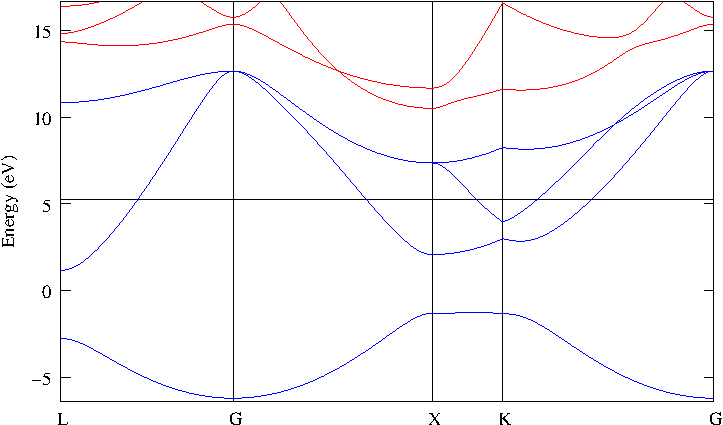
\includegraphics{lead}
\caption{Bandstructure of lead showing the position of the Fermi
  level. Only the lowest four bands are included in the calculation.} 
\label{fig:pb-bnd}
\end{center}
\end{figure}

\cleardoublepage


\sectiontitle{3: Silicon -- Disentangled MLWFs}

\begin{itemize}
\item{Outline: \it{Obtain disentangled MLWFs for the valence and
      low-lying conduction states of Si. Plot the interpolated
      bandstructure}}
\item{Generation Details: \it{From \pwscf, using norm-conserving
    pseudopotentials and a 4$\times$4$\times$4 k-point grid. Starting
    guess: atom-centred sp$^3$ hybrid orbitals}} 
\item{Directory: {\tt examples/example3/}}
\item{Input Files}
\begin{itemize}
\item{ {\tt silicon.win}  {\it The master input file}}
\item{ {\tt silicon.mmn}  {\it The overlap matrices $\Mkb$}}
\item{ {\tt silicon.amn}  {\it Projection $\Ak$ of the Bloch states onto a
    set of trial localised orbitals}} 
\item{ {\tt silicon.eig}  {\it The Bloch eigenvalues at each k-point}}
\end{itemize}
\end{itemize}
The valence and lower conduction states can be represented by MLWFs
with $sp^3$-like symmetry. The lower conduction states are not 
separated from the higher states by an energy gap. In order to form
localised WF, we use the disentanglement procedure
introduced in Ref.~\cite{souza-prb01}. The position of the inner and outer
energy windows are shown in Fig.~\ref{fig:si.bnd}. 
\begin{enumerate}
\item Run \wannier.
{\tt
\begin{quote}
wannier90.x silicon
\end{quote} }
Inspect the output file {\tt silicon.wout}. The minimisation of the
spread occurs in a two-step procedure~\cite{souza-prb01}. First, we minimise
$\Omega_{\rm I}$ -- this is the extraction of the optimal subspace in
the disentanglement procedure. Then, we minimise $\Omega_{\rm D} +
\Omega_{{\rm OD}}$.

\item Plot the energy bands by adding the following
  commands to the input file {\tt silicon.win} {\tt
\begin{quote}
restart = plot

bands\_plot = true
\end{quote} }
and re-running \wannier. The files {\tt silicon\_band.dat} and {\tt
  silicon\_band.gnu} are created. 
To plot the bandstructure using gnuplot
\smallskip
{\tt
\begin{quote}
myshell> gnuplot

gnuplot> load `silicon\_band.gnu'
\end{quote} }
The k-point path for the bandstructure interpolation is set in the {\tt
  kpoint\_path} block. Try plotting along different paths. 
\end{enumerate}

\begin{figure}[h]
\begin{center}
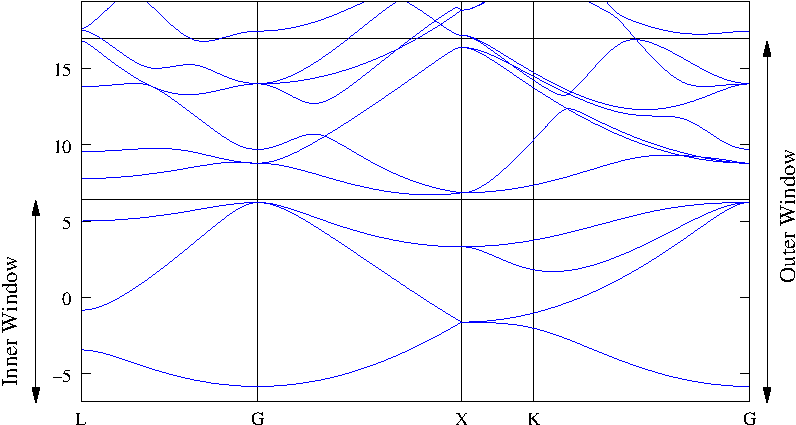
\includegraphics{si}
\caption{Bandstructure of silicon showing the position of the outer
  and inner energy windows.} 
\label{fig:si.bnd}
\end{center}
\end{figure}

\cleardoublepage


\sectiontitle{4: Copper -- Fermi surface, orbital character of energy
  bands}

\begin{itemize}
\item{Outline: \it{Obtain MLWFs to describe the states around the
    Fermi-level in copper}} 
\item{Generation Details: \it{From \pwscf, using ultrasoft
    pseudopotentials~\cite{vanderbilt-prb90} and a
    4$\times$4$\times$4 k-point grid. Starting guess: five 
    atom-centred d orbitals, and two s orbitals centred on one of each
    of the two tetrahedral interstices.}}
\item{Directory: {\tt examples/example4/}}
\item{Input Files}
\begin{itemize}
\item{ {\tt copper.win}  {\it The master input file}}
\item{ {\tt copper.mmn}  {\it The overlap matrices $\Mkb$}}
\item{ {\tt copper.amn}  {\it Projection $\Ak$ of the Bloch states onto a
    set of trial localised orbitals}} 
\item{ {\tt copper.eig}  {\it The Bloch eigenvalues at each k-point}}
\end{itemize}

\end{itemize}

\begin{enumerate}
\item Run \wannier\ to minimise the MLWFs spread
{\tt
\begin{quote}
wannier90.x copper
\end{quote} }
Inspect the output file {\tt copper.wout}. 

\item Plot the Fermi surface, it should look familiar! The Fermi
  energy is at 12.2103\,eV. 

\item Plot the interpolated bandstructure. A suitable path in k-space is
\smallskip
{\tt
\begin{quote}
begin kpoint\_path

G 0.00  0.00  0.00    X 0.50  0.50  0.00

X 0.50  0.50  0.00    W 0.50  0.75  0.25

W 0.50  0.75  0.25    L 0.00  0.50  0.00

L 0.00  0.50  0.00    G 0.00  0.00  0.00

G 0.00  0.00  0.00    K 0.00  0.50 -0.50
 
end kpoint\_path
\end{quote} }
\item Plot the contribution of the interstitial WF to the
  bandstructure. Add the following keyword to {\tt copper.win}
\smallskip
{\tt
\begin{quote}
bands\_plot\_project = 6,7
\end{quote} } The resulting file {\tt copper\_band\_proj.gnu} can be
opened with gnuplot. Red lines correspond to a large contribution from
the interstitial WF (blue line are a small contribution; ie a large
$d$ contribution).


\end{enumerate}




Investigate the effect of the outer and inner energy window on the
interpolated bands. 



\begin{figure}[h]
\begin{center}
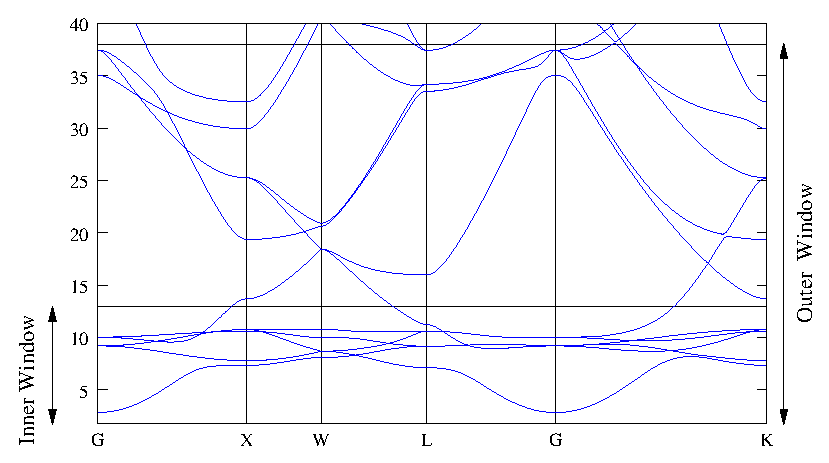
\includegraphics{cu}
\caption{Bandstructure of copper showing the position of the outer
  and inner energy windows.} 
\label{fig:cu-bnd}
\end{center}
\end{figure}

\cleardoublepage

\sectiontitle{Examples Using the {\sc pwscf} Interface}
\label{sec:using pwscf}

The \pwscf\ plane-wave, density-functional theory code, which is
available as part of the \QE\ distribution (\url{http://www.quantum-espresso.org}), is fully interfaced to \wannier\ via the
{\tt pw2wannier90} post-processing code that is also available as part
of \QE. The latest version of {\tt pw2wannier90} is included as part of 
the \wannier\ distribution. Please see the {\tt pwscf} directory for 
instructions on how to incorporate it into \pwscf. 

Note that both the {\tt PWSCF} executable {\tt pw.x} {\it and} {\tt
  pw2wannier90.x} can be run in parallel, which for large calculations
can reduce the computation time very significantly.  This requires
compiling the code in its parallel version, using the MPI
libraries. Refer to the \QE\ package for the documentation on how to
do so.  Note that, unless you specify {\tt wf\_collect=.true.} in your
{\tt pw.x} input file, you must run {\tt pw2wannier90} with the same
number of processors as {\tt pw.x}.

Moreover we remind here that, as discussed in the ``Parallel
execution'' section at page \pageref{sec:parallel}, while the
\wannier\ executable is serial-only, {\tt postw90.x} can be run in
parallel. In this case any number of processors can be used,
independently of the number used for {\tt pw.x} and {\tt
  pw2wannier90.x}.

\cleardoublepage

\sectiontitle{5: Diamond -- MLWFs for the valence bands}
\begin{itemize}
\item{Outline: \it{Obtain MLWFs for the valence bands of diamond}}
\item{Directory: {\tt examples/example5/}}
\item{Input Files}
\begin{itemize}
\item{ {\tt diamond.scf}  {\it The \pwscf\ input file for ground state
    calculation}} 
\item{ {\tt diamond.nscf}  {\it The \pwscf\ input file to obtain Bloch
    states on a uniform grid}} 
\item{ {\tt diamond.pw2wan}  {\it The input file for {\tt pw2wannier90}}}
\item{ {\tt diamond.win}  {\it The {\tt wannier90} input file}}
\end{itemize}
\end{itemize}

\begin{enumerate}
\item Run \pwscf\ to obtain the ground state of diamond\\
{\tt pw.x < diamond.scf > scf.out}

\item Run \pwscf\ to obtain the Bloch states on a uniform k-point grid\\
{\tt pw.x < diamond.nscf > nscf.out}

\item Run \wannier\ to generate a list of the required overlaps (written
  into the {\tt diamond.nnkp} file).\\ 
{\tt wannier90.x -pp diamond}

\item Run {\tt pw2wannier90} to compute the overlap between Bloch
  states and the projections for the starting guess (written in the
  {\tt diamond.mmn} and {\tt diamond.amn} files).\\  
{\tt pw2wannier90.x < diamond.pw2wan > pw2wan.out}

\item Run \wannier\ to compute the MLWFs.\\
{\tt wannier90.x diamond}
\end{enumerate}

\cleardoublepage

\sectiontitle{6: Copper -- Fermi surface}

\begin{itemize}
\item{Outline: \it{Obtain MLWFs to describe the states around the
    Fermi-level in copper}}
\item{Directory: {\tt examples/example6/}}
\item{Input Files}
\begin{itemize}
\item{ {\tt copper.scf}  {\it The \pwscf\ input file for ground state
    calculation}} 
\item{ {\tt copper.nscf}  {\it The \pwscf\ input file to obtain Bloch states
    on a uniform grid}} 
\item{ {\tt copper.pw2wan}  {\it Input file for {\tt pw2wannier90}}}
\item{ {\tt copper.win}  {\it The {\tt wannier90} input file}}
\end{itemize}

\end{itemize}

\begin{enumerate}
\item Run \pwscf\ to obtain the ground state of copper\\
{\tt pw.x < copper.scf > scf.out}

\item Run \pwscf\ to obtain the Bloch states on a uniform k-point grid\\
{\tt pw.x < copper.nscf > nscf.out}

\item Run \wannier\ to generate a list of the required overlaps (written
  into the {\tt copper.nnkp} file).\\ 
{\tt wannier90.x -pp copper}

\item Run {\tt pw2wannier90} to compute the overlap between Bloch
  states and the projections for the starting guess (written in the
  {\tt copper.mmn} and {\tt copper.amn} files).\\  
{\tt pw2wannier90.x < copper.pw2wan > pw2wan.out}

\item Run \wannier\ to compute the MLWFs.\\
{\tt wannier90.x copper}
\end{enumerate}

Inspect the output file {\tt copper.wout}. 

\begin{enumerate}
\item Use Wannier interpolation to obtain the Fermi surface of
  copper. Rather than re-running the whole calculation we can use the
  unitary transformations obtained in the first calculation and restart
  from the plotting routine. Add the following keywords to the {\tt
    copper.win} file:
{\tt
\begin{quote}
restart = plot

fermi\_energy = [insert your value here] 

fermi\_surface\_plot = true
\end{quote} } and re-run \wannier. The value of the Fermi energy can
be obtained from the initial first principles calculation. \wannier\
calculates the band energies, through wannier interpolation, on a
dense mesh of k-points in the Brillouin zone. The density of this grid
is controlled by the keyword {\tt fermi\_surface\_num\_points}. The
default value is 50 (i.e., 50$^3$ points).  The Fermi surface file
{\tt copper.bxsf} can be viewed using {\tt XCrySDen}, e.g.,
%
{\tt
\begin{quote}
xcrysden --bxsf copper.bxsf
\end{quote} }


\item Plot the interpolated bandstructure. A suitable path in k-space is
\smallskip
{\tt
\begin{quote}
begin kpoint\_path

G 0.00  0.00  0.00    X 0.50  0.50  0.00

X 0.50  0.50  0.00    W 0.50  0.75  0.25

W 0.50  0.75  0.25    L 0.00  0.50  0.00

L 0.00  0.50  0.00    G 0.00  0.00  0.00

G 0.00  0.00  0.00    K 0.00  0.50 -0.50
 
end kpoint\_path
\end{quote} }
\end{enumerate}

\subsection*{Further ideas}
\begin{itemize}
\item Compare the Wannier interpolated bandstructure with the full
  \pwscf\ bandstructure. Obtain MLWFs using a denser k-point grid.
\tent{{[Provide script for this? Link to Jonathan's URL?]}}
\item Investigate the effects of the outer and inner energy windows on
  the interpolated bands. 
\item Instead of extracting a subspace of seven states, we could
  extract a nine dimensional space (i.e., with $s$, $p$ and $d$
  character). Examine this case and compare the interpolated
  bandstructures.
\end{itemize}

%\begin{figure}[h]
%\begin{center}
%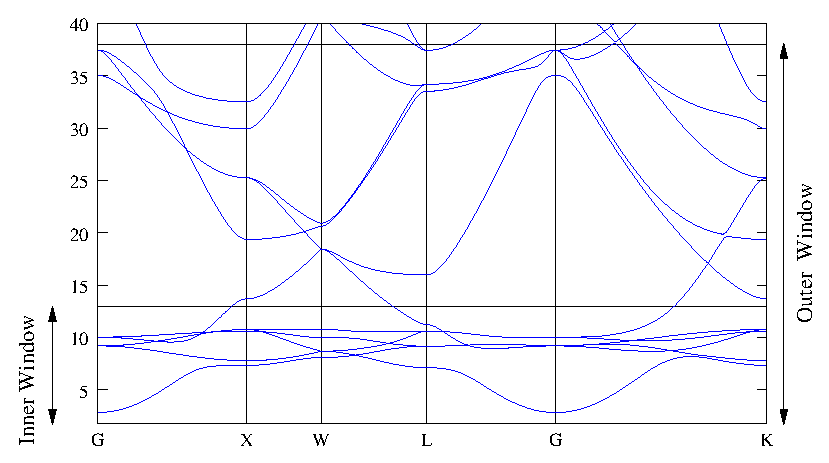
\includegraphics{cu}
%\caption{Band Structure of Copper showing the position of the outer
%  and inner energy windows.}
%\label{fig:cu-bnd}
%\end{center}
%\end{figure}

\cleardoublepage

\sectiontitle{7: Silane (SiH$_4$) -- Molecular MLWFs using
  $\Gamma$-point sampling}
\begin{itemize}
\item{Outline: \it{Obtain MLWFs for the occupied states of molecular
    silane. $\Gamma$-point sampling}} 
\item{Directory: {\tt examples/example7/}}
\item{Input Files}
\begin{itemize}
\item{ {\tt silane.scf}  {\it The \pwscf\ input file for ground state
    calculation}} 
\item{ {\tt silane.nscf}  {\it The \pwscf\ input file to obtain Bloch states
    on a uniform grid}} 
\item{ {\tt silane.pw2wan}  {\it Input file for {\tt pw2wannier90}}}
\item{ {\tt silane.win}  {\it The {\tt wannier90} input file}}
\end{itemize}
\end{itemize}

\begin{enumerate}
\item Run \pwscf\ to obtain the ground state of silane\\
{\tt pw.x < silane.scf > scf.out}

\item Run \pwscf\ to obtain the Bloch states on a uniform k-point grid\\
{\tt pw.x < silane.nscf > nscf.out}

\item Run \wannier\ to generate a list of the required overlaps (written
  into the {\tt silane.nnkp} file).\\ 
{\tt wannier90.x -pp silane}

\item Run {\tt pw2wannier90} to compute the overlap between Bloch
  states and the projections for the starting guess (written in the
  {\tt silane.mmn} and {\tt silane.amn} files).\\  
{\tt pw2wannier90.x < silane.pw2wan > pw2wan.out}

\item Run \wannier\ to compute the MLWFs.\\
{\tt wannier90.x silane}
\end{enumerate}

\cleardoublepage

\sectiontitle{8: Iron -- Spin-polarized WFs, DOS, projected WFs versus MLWFs}
\begin{itemize}
\item{Outline: \it{Generate both maximally-localized and projected
      Wannier functions for ferromagnetic bcc Fe. Calculate the total
      and orbital-projected density of states by Wannier
      interpolation.}}
\item{Directory: {\tt examples/example8/}}
\item{Input Files}
\begin{itemize}
\item{ {\tt iron.scf} {\it The \pwscf\ input file for the
      spin-polarized ground state calculation}}
\item{ {\tt iron.nscf}  {\it The \pwscf\ input file to obtain Bloch states
    on a uniform grid}} 
\item{ {\tt iron\_\{up,down\}.pw2wan}  {\it Input files for {\tt pw2wannier90}}} 
\item{ {\tt iron\_\{up,down\}.win} {\it Input files for {\tt wannier90} and {\tt
          postw90}}}
\end{itemize}
\item{Note that in a spin-polarized calculation the spin-up and
    spin-down MLWFs are computed separately. (The more general case of
    spinor WFs will be treated in Example~17.)}
\end{itemize}

\begin{enumerate}
\item Run \pwscf\ to obtain the ferromagnetic ground state of bcc Fe\\
{\tt pw.x < iron.scf > scf.out}

\item Run \pwscf\ to obtain the Bloch states on a uniform k-point grid\\
{\tt pw.x < iron.nscf > nscf.out}

\item Run \wannier\ to generate a list of the required overlaps (written
  into the {\tt .nnkp} files).\\
{\tt wannier90.x -pp iron\_up}\\
{\tt wannier90.x -pp iron\_dn}

\item Run {\tt pw2wannier90} to compute the overlap between Bloch
  states and the projections for the starting guess (written in the
  {\tt .mmn} and {\tt .amn} files).\\
  {\tt pw2wannier90.x < iron\_up.pw2wan > pw2wan\_up.out}\\
  {\tt pw2wannier90.x < iron\_dn.pw2wan > pw2wan\_dn.out}

\item Run \wannier\ to compute the MLWFs.\\
{\tt wannier90.x iron\_up}\\
{\tt wannier90.x iron\_dn}

\end{enumerate}

\subsection*{Density of states}

To compute the DOS using a $25\times 25 \times 25$ $k$-point grid add
to the two {\tt .win} files
%
{\tt
\begin{quote}
dos = true

dos\_kmesh = 25
\end{quote}
}
%
run {\tt postw90},
%
{\tt
\begin{quote}
postw90.x iron\_up

postw90.x iron\_dn
\end{quote}
}
%
and plot the DOS with {\tt gnuplot},
%
{\tt
\begin{quote}
myshell> gnuplot

gnuplot> plot `iron\_up\_dos.dat' u (-\$2):(\$1-12.6256) w l,`iron\_dn\_dos.dat' u 2:(\$1-12.6256) w l

\end{quote} 
}
%
Energies are referred to the Fermi level (12.6256~eV, from {\tt
  scf.out}).  Note the exchange splitting between the up-spin and
down-spin DOS. Check the convergence by repeating the DOS calculations
with more $k$-points.

\subsection*{Projected versus maximally-localized Wannier functions}

In the calculations above we chose $s$, $p$, and $d$-type trial
orbitals in the {\tt .win} files,
%
{\tt
\begin{quote}
Fe:s;p;d
\end{quote}
}
%
Let us analyze the evolution of the WFs during the gauge-selection
step. Open one of the {\tt .wout} files and search for ``{\tt Initial
  state}''; those are the {\it projected} WFs. As expected they are
atom-centered, with spreads organized in three groups, 1+3+5: one $s$,
three $p$, and five $d$.  Now look at the final state towards the end
of the file.  The Wannier spreads have re-organized in two groups,
6+3; moreover, the six more diffuse WFs are off-centered: the initial
atomic-like orbitals hybridized with one another, becoming more
localized in the process. It is instructive to visualize the
final-state MLWFs using {\tt XCrySDen}, following Example~1. For more
details, see Sec.~IV.B of Ref.~\cite{wang-prb06}.

Let us plot the evolution of the spread functional~$\Omega$,
%
{\tt
\begin{quote}
myshell> grep SPRD iron\_up.wout > sprd\_up

myshell> gnuplot

gnuplot> plot `sprd\_up' u 6  w l
\end{quote}
}

\begin{figure}[h]
\begin{center}
\scalebox{0.35}{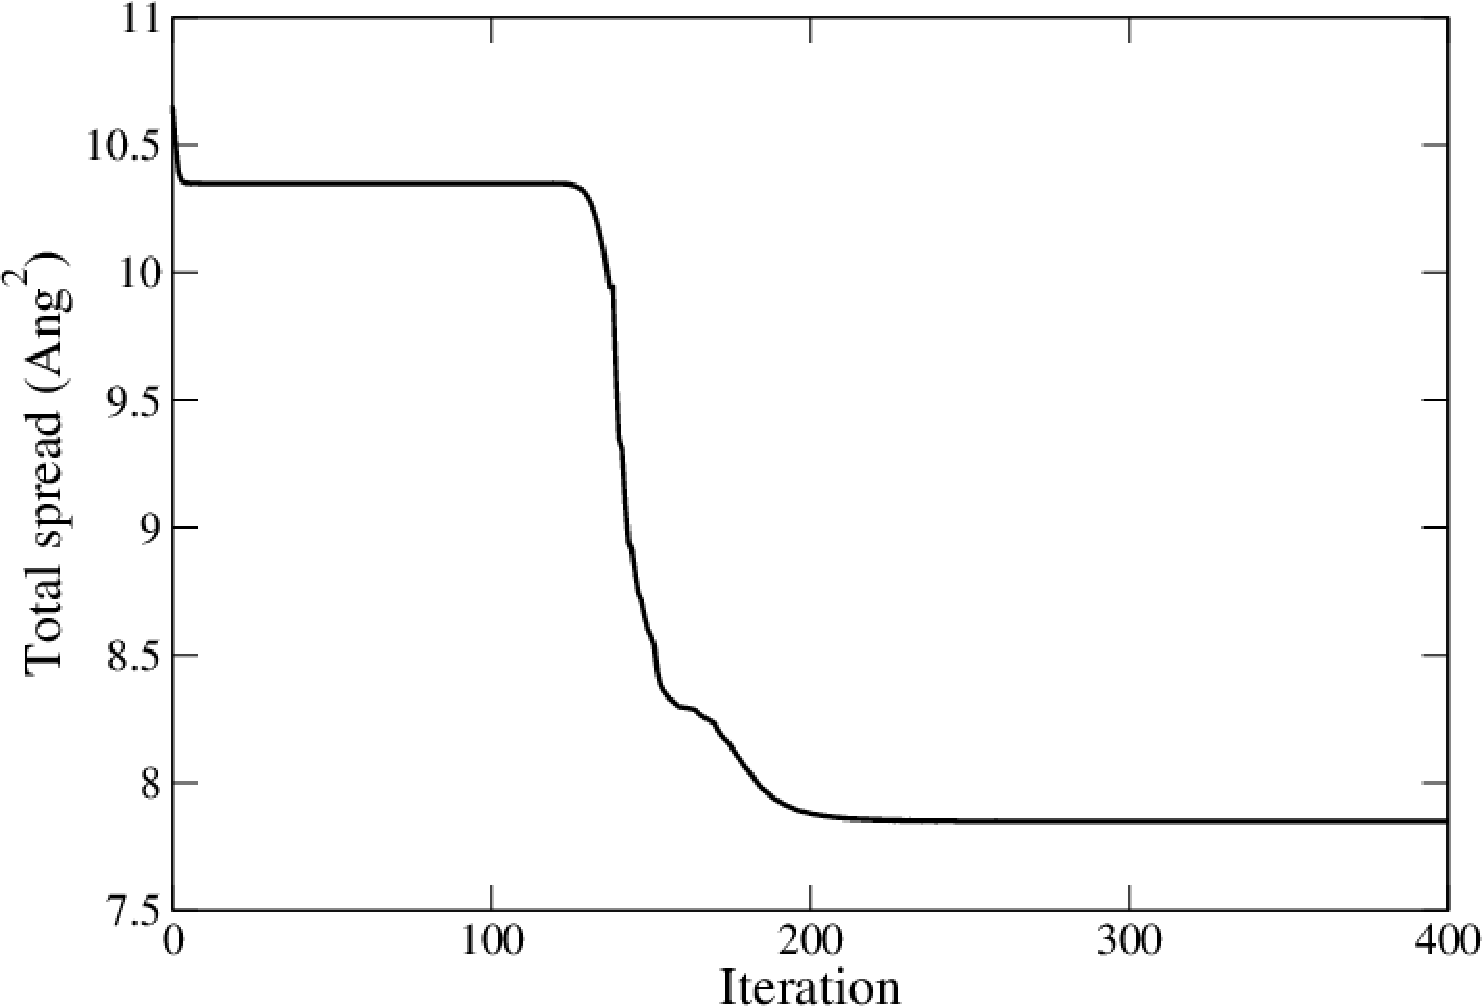
\includegraphics{Fe-spread}}
\caption{Evolution of the Wannier spread $\Omega$ of the minority
  (spin-up) bands of bcc Fe during the iterative minimization of
  $\widetilde{\Omega}$, starting from $s$, $p$, and $d$-type trial
  orbitals.}
\label{fig:Fe-sprd}
\end{center}
\end{figure}


The first plateau corresponds to atom-centered WFs of separate $s$,
$p$, and $d$ character, and the sharp drop signals the onset of the
hybridization. With hindsight, we can redo steps~4 and~5 more
efficiently using trial orbitals with the same character as the final
MLWFs,
%
{\tt
\begin{quote}
Fe:sp3d2;dxy;dxz,dyz
\end{quote}
}
%
With this choice the minimization converges much more rapidly.

Any reasonable set of localized WFs spanning the states of interest
can be used to compute physical quantities (they are
``gauge-invariant''). Let us recompute the DOS using, instead of
MLWFs, the WFs obtained by projecting onto $s$, $p$, and $d$-type
trial orbitals, without further iterative minimization of the spread
functional. This can be done by setting
%
{\tt
\begin{quote}
num\_iter = 0
\end{quote}
}
%
\tent{[But note that we still need to do disentanglement!]}
Recalculate the DOS to confirm that it is almost identical to the one
obtained earlier using the hybridized set of MLWFs. Visualize the
projected WFs using {\tt XCrySDen}, to see that they retain the pure
orbital character of the individual trial orbitals.


\subsection*{Orbital-projected DOS and exchange splitting}

With projected WFs the total DOS can be separated into $s$, $p$ and
$d$ contributions, in a similar way to the orbital decomposition of
the energy bands in Example~4.
  
In order to obtain the partial DOS projected onto the $p$-type WFs,
add to the {\tt .win} files
%
{\tt
\begin{quote}
dos\_project = 2,3,4
\end{quote}
}
%
and re-run {\tt postw90}. Plot the projected DOS for both up- and
down-spin bands. Repeat for the $s$ and $d$ projections. 

Projected WFs can also be used to quantify more precisely the exchange
splitting between majority and minority states. Re-run {\tt wannier90}
after setting {\tt dos=false} and adding to the {\tt .win} files
%
{\tt
\begin{quote}
write\_hr\_diag = true
\end{quote}
}
%
This instructs {\tt wannier90} to print in the output file the on-site
energies $\langle {\bf 0}n\vert H\vert {\bf 0}n\rangle$. The
difference between corresponding values in {\tt iron\_up.wout} and in
{\tt iron\_dn.wout} gives the exchange splittings for the individual
orbitals. Compare their magnitudes with the splittings displayed by
the orbital-projected DOS plots.  In agreement with the Stoner
criterion, the largest exchange splittings occur for the localized
$d$-states, which contribute most of the density of states at the
Fermi level.


\cleardoublepage


\sectiontitle{9: Cubic BaTiO$_3$}
\begin{itemize}
\item{Outline: \it{Obtain MLWFs for a perovskite}}
\item{Directory: {\tt examples/example9/}}
\item{Input Files}
\begin{itemize}
\item{ {\tt batio3.scf}  {\it The \pwscf\ input file for ground state
    calculation}} 
\item{ {\tt batio3.nscf}  {\it The \pwscf\ input file to obtain Bloch states
    on a uniform grid}} 
\item{ {\tt batio3.pw2wan}  {\it Input file for {\tt pw2wannier90}}}
\item{ {\tt  batio3.win}  {\it The {\tt wannier90} input file}}
\end{itemize}
\end{itemize}

 To start with, we are going to obtain MLWFs for the oxygen 2p
  states. From the bandstructure~\cite{marzari-arxiv98}, these form an isolated
  group of bands. We use the \wannier\ keyword {\tt exclude\_bands} to
  remove all but the 2p bands from the calculation of the overlap
  and projection matrices (we don't have to do this, but it saves time).

\begin{enumerate}
\item Run \pwscf\ to obtain the ground state of BaTiO$_3$\\
{\tt pw.x < BaTiO3.scf > scf.out}

\item Run \pwscf\ to obtain the Bloch states on a uniform k-point grid\\
{\tt pw.x < BaTiO3.nscf > nscf.out}

\item Run \wannier\ to generate a list of the required overlaps (written
  into the {\tt BaTiO3.nnkp} file).\\ 
{\tt wannier90.x -pp BaTiO3}

\item Run {\tt pw2wannier90} to compute the overlap between Bloch
  states and the projections for the starting guess (written in the
  {\tt BaTiO3.mmn} and {\tt BaTiO3.amn} files).\\  
{\tt pw2wannier90.x < BaTiO3.pw2wan > pw2wan.out}

\item Run \wannier\ to compute the MLWFs.\\
{\tt wannier90.x BaTiO3}
\end{enumerate}

Inspect the output file {\tt BaTiO3.wout}. 

Plot the second MLWF, as described in Section~1, by adding the
following keywords to the input file {\tt BaTiO3.win}
{\tt
\begin{quote}
wannier\_plot = true\\
restart = plot\\
wannier\_plot\_list = 2\\
wannier\_plot\_supercell = 3
\end{quote} }
and re-running \wannier. Visualise it using {\tt XCrySDen},
{\tt
\begin{quote}
xcrysden --xsf BaTiO3\_00002.xsf
\end{quote} }

We can now simulate the ferroelectric phase by displacing the Ti
  atom. Change its position to 
{\tt
\begin{quote}
Ti 0.505 0.5 0.5
\end{quote}
}
and regenerate the MLWFs (i.e., compute the ground-state charge
density and Bloch states using \pwscf, etc.) and look at the change in
the second MLWF.

\subsection*{Further ideas}
\begin{itemize}
\item Look at MLWFs for other groups of bands. What happens if you form
  MLWFs for the whole valence manifold?

\item Following Ref.~\cite{marzari-arxiv98}, compute the Born effective charges from the
  change in Wannier centres under an atomic displacement. 
\end{itemize}

\cleardoublepage

\sectiontitle{10: Graphite}
\begin{itemize}
\item{Outline: \it{Obtain MLWFs for graphite (AB, Bernal)}}
\item{Directory: {\tt examples/example10/}}
\item{Input Files}
\begin{itemize}
\item{ {\tt graphite.scf}  {\it The \pwscf\ input file for ground
    state calculation}} 
\item{ {\tt graphite.nscf}  {\it The \pwscf\ input file to obtain Bloch
    states on a uniform grid}} 
\item{ {\tt graphite.pw2wan}  {\it Input file for {\tt pw2wannier90}}}
\item{ {\tt graphite.win}  {\it The {\tt wannier90} input file}}
\end{itemize}
\end{itemize}

\begin{enumerate}
\item Run \pwscf\ to obtain the ground state of graphite\\
{\tt pw.x < graphite.scf > scf.out}

\item Run \pwscf\ to obtain the Bloch states on a uniform k-point grid\\
{\tt pw.x < graphite.nscf > nscf.out}

\item Run \wannier\ to generate a list of the required overlaps (written
  into the {\tt graphite.nnkp} file).\\ 
{\tt wannier90.x -pp graphite}

\item Run {\tt pw2wannier90} to compute the overlap between Bloch
  states and the projections for the starting guess (written in the
  {\tt graphite.mmn} and {\tt graphite.amn} files).\\  
{\tt pw2wannier90.x < graphite.pw2wan > pw2wan.out}

\item Run \wannier\ to compute the MLWFs.\\
{\tt wannier90.x graphite}
\end{enumerate}


\cleardoublepage


\sectiontitle{11: Silicon -- Valence and conduction states, scissors
  correction}
\subsection*{Valence States}
\begin{itemize}
\item{Outline: \it{Obtain MLWFs for the valence bands of silicon.}}
\item{Directory: {\tt examples/example11/}}
\item{Input Files}
\begin{itemize}
\item{ {\tt silicon.scf}  {\it The \pwscf\ input file for ground state
    calculation}} 
\item{ {\tt silicon.nscf}  {\it The \pwscf\ input file to obtain Bloch
    states on a uniform grid}} 
\item{ {\tt silicon.pw2wan}  {\it Input file for {\tt pw2wannier90}}}
\item{ {\tt silicon.win}  {\it The {\tt wannier90} input file}}
\end{itemize}

\end{itemize}

\begin{enumerate}
\item Run \pwscf\ to obtain the ground state of silicon\\
{\tt pw.x < silicon.scf > scf.out}

\item Run \pwscf\ to obtain the Bloch states on a uniform k-point
  grid. Note that we request the lower 4 (valence) bands\\ 
{\tt pw.x < silicon.nscf > nscf.out}

\item Run \wannier\ to generate a list of the required overlaps (written
  into the {\tt silicon.nnkp} file).\\
{\tt wannier90.x -pp silicon}

\item Run {\tt pw2wannier90} to compute the overlap between Bloch
  states and the projections for the starting guess (written in the
  {\tt silicon.mmn} and {\tt  silicon.amn} files).\\
{\tt pw2wannier90.x < silicon.pw2wan > pw2wan.out}

\item Run \wannier\ to compute the MLWFs.\\
{\tt wannier90.x silicon}

\end{enumerate}

Inspect the output file {\tt silicon.wout}. The total spread converges to its
minimum value after just a few iterations. Note that the geometric centre of
each MLWF lies at the centre of the Si-Si bond.
Note also that the memory requirement for the minimisation of
the spread is very low as the MLWFs are defined 
by just the 4$\times$4 unitary matrices $\Uk$. 

Plot the MLWFs by adding the following keywords to the input file {\tt
  silicon.win} 
{\tt
\begin{quote}
wannier\_plot = true
\end{quote} }
and re-running \wannier. Visualise them using {\tt XCrySDen}, e.g.,
{\tt
\begin{quote}
xcrysden --xsf silicon\_00001.xsf
\end{quote} }

\subsection*{Valence + Conduction States}

\begin{itemize}
\item{Outline: \it{Obtain MLWFs for the valence and low-lying
      conduction-band states of Si. Plot the interpolated
      bandstructure. Apply a scissors correction to the conduction
      bands.}}
\item{Input Files}
\begin{itemize}
\item{ {\tt silicon.scf}  {\it The \pwscf\ input file for ground state
    calculation}} 
\item{ {\tt silicon.nscf}  {\it The \pwscf\ input file to obtain Bloch
    states on a uniform grid}} 
\item{ {\tt silicon.pw2wan}  {\it Input file for {\tt pw2wannier90}}}
\item{ {\tt silicon.win}  {\it The {\tt wannier90} input file}}
\end{itemize}
\end{itemize}
The valence and lower conduction states can be represented by MLWFs
with $sp^3$-like symmetry. The lower conduction states are not
separated by an energy gap from the higher states. In order to form
localised WF we use the disentanglement procedure introduced in
Ref.~\cite{souza-prb01}. The position of the inner and outer energy
windows are shown in Fig.~\ref{fig:si.bnd}.
\begin{enumerate}
\item Modify the input file and run \pwscf\ and \wannier.\\
Inspect the output file {\tt silicon.wout}. The minimisation of the
spread occurs in a two-step procedure. First, we minimise $\Omega_{\rm
  I}$ -- this is the extraction of the optimal subspace in the 
disentanglement procedure. Then, we minimise $\Omega_{\rm
  O}+\Omega_{{\rm OD}}$.

\item Plot the bandstructure by adding the following commands to the
 input file {\tt silicon.win}
{\tt
\begin{quote}
restart = plot

bands\_plot = true
\end{quote} }
and re-running \wannier. The files {\tt silicon\_band.dat} and {\tt
  silicon\_band.gnu} are created. To plot the bandstructure using
  gnuplot \smallskip
{\tt
\begin{quote}
myshell> gnuplot

gnuplot> load `silicon\_band.gnu'
\end{quote} }
The k-point path for the bandstructure interpolation is set in the {\tt
  kpoint\_path} block. Try plotting along different paths. 

\item Shift the conduction bands upwards in energy by
    0.65~eV. This {\it ad-hoc} ``scissors correction'' is applied to
    the Hamiltonian in the Wannier basis using the instructions
%
{\tt
\begin{quote}
num\_valence\_bands = 4

scissors\_shift = 0.65
\end{quote} }
%
Plot together the original and scissors-corrected bands.

\end{enumerate}

\subsection*{Further ideas}

\begin{itemize}
\item Compare the Wannier-interpolated bandstructure with the full
  \pwscf\ bandstructure. Recompute the MLWFs using a finer $k$-point
  grid (e.g., 6$\times$6$\times$6 or 8$\times$8$\times$8) and note how
  the accuracy of the interpolation increases~\cite{yates-prb07}.
\item Compute four MLWFs spanning the low-lying conduction states (see
  Ref.~\cite{souza-prb01}).
\end{itemize}

%\begin{figure}[h]
%\begin{center}
%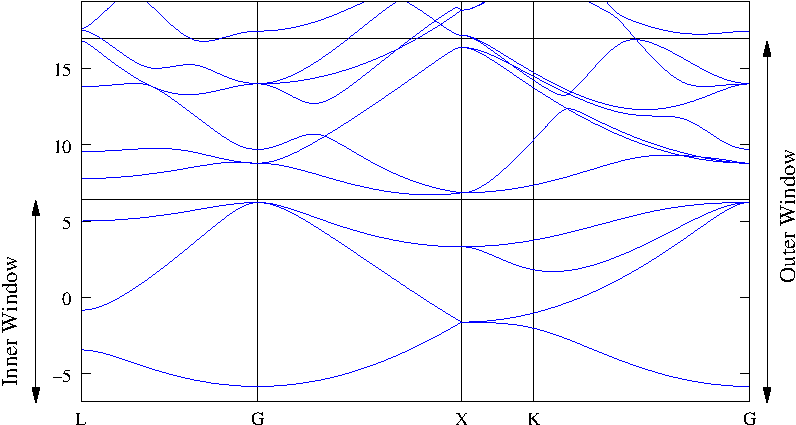
\includegraphics{si}
%\caption{Band Structure of Silicon showing the position of the outer
%and inner energy windows.}
%\label{fig:si.bnd}
%\end{center}
%\end{figure}

\cleardoublepage


\sectiontitle{12: Benzene}
\subsection*{Valence States}
\begin{itemize}
\item{Outline: \it{Obtain MLWFs for the valence states of benzene}}
\item{Directory: {\tt examples/example12/}}
\item{Input Files}
\begin{itemize}
\item{ {\tt benzene.scf}  {\it The \pwscf\ input file for ground state
    calculation}} 
\item{ {\tt benzene.pw2wan}  {\it Input file for {\tt pw2wannier90}}}
\item{ {\tt benzene.win}  {\it The {\tt wannier90} input file}}
\end{itemize}

\end{itemize}

\begin{enumerate}
\item Run \pwscf\ to obtain the ground state of benzene\\
{\tt pw.x < benzene.scf > scf.out}

\item Run \wannier\ to generate a list of the required overlaps (written
  into the {\tt benzene.nnkp} file).\\
{\tt wannier90.x -pp benzene}

\item Run {\tt pw2wannier90} to compute the overlap between Bloch
  states and the projections for the starting guess (written in the
  {\tt benzene.mmn} and {\tt  benzene.amn} files).\\
{\tt pw2wannier90.x < benzene.pw2wan > pw2wan.out}

\item Run \wannier\ to compute the MLWFs.\\
{\tt wannier90.x benzene}

\end{enumerate}

Inspect the output file {\tt benzene.wout}. The total spread converges
to its minimum value after just a few iterations. 

Plot the MLWFs by adding the following keywords to the input file {\tt
  benzene.win} 
{\tt
\begin{quote}
restart               = plot\\
wannier\_plot         = true\\
wannier\_plot\_format = cube\\
wannier\_plot\_list   = 2-4
\end{quote} }
and re-running \wannier. Visualise them using, e.g., {\tt XCrySDen}. 

\subsection*{Valence + Conduction States}

\begin{itemize}
\item{Outline: \it{Obtain MLWFs for the valence and low-lying
    conduction states of benzene.}} 
\item{Input Files}
\begin{itemize}
\item{ {\tt benzene.scf}  {\it The \pwscf\ input file for ground state
    calculation}} 
\item{ {\tt benzene.nscf}  {\it The \pwscf\ input file to obtain Bloch
    states for the conduction states}} 
\item{ {\tt benzene.pw2wan}  {\it Input file for {\tt pw2wannier90}}}
\item{ {\tt benzene.win}  {\it The {\tt wannier90} input file}}
\end{itemize}
\end{itemize}
In order to form localised WF we use the disentanglement
procedure. The position of the inner energy window is set to lie in
the energy gap; the outer energy window is set to 4.0\,eV. Modify the
input file appropriately. 
\begin{enumerate}
\item Run \pwscf\ and \wannier.\\
Inspect the output file {\tt benzene.wout}. The minimisation of the
spread occurs in a two-step procedure. First, we minimise $\Omega_{\rm
  I}$. Then, we minimise $\Omega_{\rm O}+\Omega_{{\rm OD}}$.

\item Plot the MLWFs by adding the following commands to the
 input file {\tt benzene.win}
{\tt
\begin{quote}
restart               = plot\\
wannier\_plot         = true\\
wannier\_plot\_format = cube\\
wannier\_plot\_list   = 1,7,13
\end{quote} }
and re-running \wannier. Visualise them using, e.g., {\tt XCrySDen}. 
\end{enumerate}

\cleardoublepage

\sectiontitle{13: (5,5) Carbon Nanotube -- Transport properties}
%\subsection*{Transport properties}

\begin{itemize}
  \item{Outline: \it{Obtain the bandstructure, quantum conductance and
  density of states of a metallic (5,5) carbon nanotube}}
  \item{Directory: {\tt examples/example13/}}
  \item{Input Files}
    \begin{itemize}
      \item{ {\tt cnt55.scf}  {\it The \pwscf\ input file for ground state
	  calculation}}
      \item{ {\tt cnt55.nscf}  {\it The \pwscf\ input file to obtain Bloch
	  states for the conduction states}} 
      \item{ {\tt cnt55.pw2wan}  {\it Input file for {\tt pw2wannier90}}}
      \item{ {\tt cnt55.win}  {\it The {\tt wannier90} input file}}
    \end{itemize}
\end{itemize}

In order to form localised WF that describe both the occupied and
unoccupied $\pi$ and $\pi^{\ast}$ manifolds, we use the
disentanglement procedure to extract a smooth manifold of states that
has dimension equal to 2.5 times the number of carbon atoms per unit
cell~\cite{lee-prl05}. The positions of the energy windows are shown in
Fig.~\ref{fig:cnt.win}.

The part of the \wannier\ input file that controls the transport part
of the calculation looks like:

{\tt
\begin{quote}
transport                 = true\\
transport\_mode           = bulk\\
one\_dim\_axis            = z\\
dist\_cutoff              =  5.5\\
fermi\_energy             = -1.06\\
tran\_win\_min            = -6.5\\
tran\_win\_max            = 6.5\\
tran\_energy\_step         = 0.01\\
dist\_cutoff\_mode        = one\_dim\\
translation\_centre\_frac = 0.0 0.0 0.0
\end{quote} }

Descriptions of these and other keywords related to the calculation of
transport properties can be found in the User Guide.

\begin{enumerate}
\item Run \pwscf\ and \wannier.\\
Inspect the output file {\tt cnt55.wout}. The minimisation of the
spread occurs in a two-step procedure. First, we minimise $\Omega_{\rm
  I}$. Then, we minimise $\Omega_{\rm O}+\Omega_{{\rm OD}}$.
\item Note that the initial $p_{z}$ projections on the carbon atoms
are oriented in the radial direction with respect to the nanotube
axis.
\item The interpolated bandstructure is written to {\tt
cnt55\_band.agr} (since {\tt bands\_plot\_format = xmgr} in the input
file).
\item The quantum conductance and density of states are written to the
files {\tt cnt55\_qc.dat} and {\tt cnt55\_dos.dat}, respectively. 
Note that this part of the calculation may take some time. You can 
follow its progress by monitoring the output to these files. 
Use a package such as {\tt gnuplot} or {\tt xmgrace} in order to visualise
the data. You should get something that looks like Fig.~\ref{fig:cnt.tran}.
\end{enumerate}

\begin{figure}[h]
\begin{center}
\includegraphics[width=10cm]{cnt_win}
\caption{Bandstructure of (5,5) carbon nanotube showing the position
  of the outer and inner energy windows.}
\label{fig:cnt.win}
\end{center}
\end{figure}

\begin{figure}[h]
\begin{center}
\scalebox{0.8}{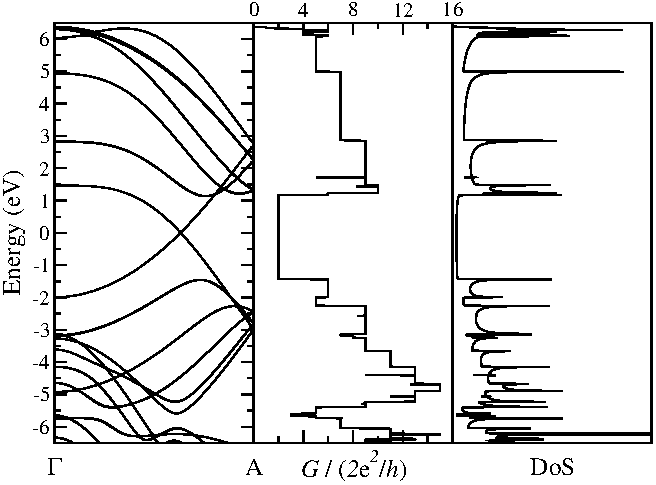
\includegraphics{cnt_tran}}
\caption{Wannier interpolated bandstructure, quantum conductance and
density of states of (5,5) carbon nanotube. Note that the Fermi level has been shifted 
by 1.06eV with respect to Fig.~\ref{fig:cnt.win}.}
\label{fig:cnt.tran}
\end{center}
\end{figure}

\cleardoublepage

\sectiontitle{14: Linear Sodium Chain -- Transport properties}

\begin{itemize}
  \item{Outline: \it{Compare the quantum conductance of a periodic 
  	linear chain of Sodium atoms with that of a defected chain}}
  \item{\begin{tabbing}
  Directories: \= {\tt examples/example14/periodic}\\ 
    				 \> {\tt examples/example14/defected}
    		\end{tabbing}}
  \item{Input Files}
    \begin{itemize}
      \item{ {\tt Na\_chain.scf}  {\it The \pwscf\ input file for ground state
	  calculation}}
      \item{ {\tt Na\_chain.nscf}  {\it The \pwscf\ input file to obtain Bloch
	  states for the conduction states}} 
      \item{ {\tt Na\_chain.pw2wan}  {\it Input file for {\tt pw2wannier90}}}
      \item{ {\tt Na\_chain.win}  {\it The {\tt wannier90} input file}}
    \end{itemize}
\end{itemize}

The periodic system contains two unit cells evenly distributed along
the supercell. Transport calculations are performed using {\tt
  transport\_mode = bulk} and so the resulting quantum conductance
represents that of an infinite periodic chain.

The part of the \wannier\ input file that controls the transport part
of the calculation looks like:

{\tt
\begin{quote}
transport = true\\
transport\_mode = bulk\\
tran\_read\_ht = false\\
one\_dim\_axis = x\\
fermi\_energy = -2.7401\\
tran\_win\_min = -5.0\\
tran\_win\_max = 5.0\\
tran\_energy\_step = 0.01\\
translation\_centre\_frac = 0.5 0.5 0.5\\
tran\_num\_bb = 2

\end{quote} }

The defected system uses a 13 atom supercell with the central atom
position altered to break symmetry. Setting {\tt transport\_mode = lcr} with tell 
\wannier\ to treat the system as an infinte sytsem with the defect at its centre.
The supercell is chosen so that is conforms to the 2c2 geometry (see User Guide 
for details). Each principal layer is 2 atoms long so that the conductor 
region contains the defected atom plus a single atom on either side.

The transport section of the input file contians  these key differences:

{\tt
\begin{quote}
transport\_mode = lcr\\
tran\_num\_ll = 2\\
tran\_num\_cell\_ll = 2\\

\end{quote} }

Descriptions of these and other keywords related to the calculation of
transport properties can be found in the User Guide.

\begin{enumerate}
\item Run \pwscf\ and \wannier\ for the periodic system.
\item Run \pwscf\ and \wannier\ for the defected system.
\item The quantum conductance is written to the files {\tt periodic/Na\_chain\_qc.dat} 
and \linebreak{\tt defected/Na\_chain\_dos.dat}, respectively. 
Compare the quantum conductance of the periodic (bulk) calculation with the
defected (LCR) calculation. Your plot should look like Fig.~\ref{fig:Na_qc}.
\end{enumerate}


\begin{figure}[h]
\begin{center}
\scalebox{0.3}{\includegraphics{Na_qc}}
\caption{Quantum conductance of periodic Sodium chain (black) compared to that of the defected Sodium chain (red).}
\label{fig:Na_qc}
\end{center}
\end{figure}

\cleardoublepage

\sectiontitle{15: (5,0) Carbon Nanotube -- Transport properties}

\emph{Note that these systems require reasonably large-scale electronic 
structure calculations.}

\subsection*{Bulk Transport properties}

\begin{itemize}
  \item{Outline: \it{Obtain the quantum conductance of a pristine single-walled carbon nanotube}}
  \item{Directory: {\tt examples/example14/periodic}}
  \item{Input Files}
    \begin{itemize}
      \item{ {\tt cnt.scf}  {\it The \pwscf\ input file for ground state
	  calculation}}
      \item{ {\tt cnt.nscf}  {\it The \pwscf\ input file to obtain Bloch
	  states for the conduction states}} 
      \item{ {\tt cnt.pw2wan}  {\it Input file for {\tt pw2wannier90}}}
      \item{ {\tt cnt.win}  {\it The {\tt wannier90} input file}}
    \end{itemize}
\end{itemize}


First we consider a single unit cell, with 10 k-points. With 
{\tt transport\_mode = bulk} we compute the transport properties 
of a pristine, infinite, periodic (5,0) carbon nanotube. Later, we will 
compare the quantum conductance of this system with a defected
nanotube.

\begin{enumerate}
\item Run \pwscf\ and \wannier.\\ 
\item The quantum conductance and density of states are written to the
files {\tt cnt\_qc.dat} and {\tt cnt\_dos.dat}, respectively.
\end{enumerate}

\subsection*{LCR transport properties -- Defected nanotube}

\begin{itemize}
  \item{Outline: \it{Use the automated LCR routine to investigate the effect of
  a single silicon atom in a infinite (5,0) carbon nanotube.}}
  \item{Directory: {\tt examples/example15/defected}}
  \item{Input Files}
    \begin{itemize}
      \item{ {\tt cnt+si.scf}  {\it The \pwscf\ input file for ground state
	  calculation}}
      \item{ {\tt cnt+si.nscf}  {\it The \pwscf\ input file to obtain Bloch
	  states for the conduction states}} 
      \item{ {\tt cnt+si.pw2wan}  {\it Input file for {\tt pw2wannier90}}}
      \item{ {\tt cnt+si.win}  {\it The {\tt wannier90} input file}}
    \end{itemize}
\end{itemize}

In this calculation an 11-atom supercell is used with a single silicon
substitutional defect in the central unit cell. The supercell is
chosen so that is conforms to the 2c2 geometry (see User Guide for
details) with principal layers set to be two unit cells long.

\begin{enumerate}
\item Run \pwscf\ and \wannier. Again these are large calculations, progress
can be monitored by viewing respective output files.\\
\item The quantum conductance is written to {\tt cnt+si\_qc.dat}. 
Compare the quantum conductance with the periodic (bulk) calculation.
Your plot should look like Fig.~\ref{fig:cnt_qc}.

\end{enumerate}

\begin{figure}[h]
\begin{center}
\scalebox{0.3}{\includegraphics{cnt_qc}}
\caption{Quantum conductance of infinite pristine nanotube (black) 
compared to that of the infinite nanotube with the substitutional silicon 
defect (red).}
\label{fig:cnt_qc}
\end{center}
\end{figure}

\subsection*{Further ideas}
\begin{itemize}
\item Set {\tt hr\_plot = true} in the bulk case. Consider the magnitude of Hamiltonian 
	elements between Wannier functions in increasingly distant unit cells. Are two 
	unit cell principal layers really large enough, or are significant errors introduced?
\item Does one unit cell either side of the defected unit cell shield the disorder
	so that the leads are ideal? Does the quantum conductance change if these 
	`buffer' regions are increased?
\end{itemize}

\cleardoublepage

\sectiontitle{16: Silicon -- Boltzmann transport}
\begin{itemize}
\item{Outline: \it{Obtain MLWFs for the valence and low-lying
    conduction states of Si. Calculate the electrical conductivity, the
    Seebeck coefficient and the thermal conductivity in the constant
    relaxation time approximation using the \bw\ module.}} 
\item{Directory: {\tt examples/example16/}}
\item{Input Files}
\begin{itemize}
\item{ {\tt Si.scf}  {\it The \pwscf\ input file for ground state
    calculation}} 
\item{ {\tt Si.nscf}  {\it The \pwscf\ input file to obtain Bloch
    states on a uniform grid}} 
\item{ {\tt Si.pw2wan}  {\it Input file for {\tt pw2wannier90}}}
\item{ {\tt Si.win}  {\it The \wannier\ and \postw\ input file}}
\end{itemize}

\end{itemize}

Note the first five steps in the following are the same of Example~11.
If you have already run Example~11 (in particular, the section ``\emph{Valence + Conduction States}'')
you can start from those files and continue from point 6, after having
added the \bw\ flags to the input file.

Note that in the following, steps 1, 2, 4 and 6 can be possibly run in parallel
on multiple processors (using {\tt mpirun}), while steps 3 and 5 must
be run in serial.

\begin{enumerate}
\item Run \pwscf\ to obtain the ground state of silicon\\
{\tt pw.x < Si.scf > scf.out}

\item Run \pwscf\ to obtain the Bloch states on a uniform k-point
  grid. Details on the disentanglement procedure are discussed in Example~11.\\ 
{\tt pw.x < Si.nscf > nscf.out}

\item Run \wannier\ to generate a list of the required overlaps (written
  into the {\tt Si.nnkp} file).\\
{\tt wannier90.x -pp Si}

\item Run {\tt pw2wannier90} to compute the overlap between Bloch
  states and the projections for the starting guess (written in the
  {\tt Si.mmn} and {\tt  Si.amn} files).\\
{\tt pw2wannier90.x < Si.pw2wan > pw2wan.out}

\item Run \wannier\ to compute the MLWFs.\\
{\tt wannier90.x Si}

Inspect the output file {\tt Si.wout} and check if the convergence was reached both in the
disentanglement and in the wannierisation steps (as discussed in further detail in Example~11).
You may also want to plot the Wannier functions and the interpolated band structure.

\item Run \postw\ to calculate the transport coefficients.\\
{\tt postw90.x Si} (serial execution) \\
{\tt mpirun -np 8 postw90.x Si} (example of parallel execution with 8 nodes) 
\end{enumerate}

Inspect the output file {\tt Si.wpout}. It summarizes the main details of the calculation (more details can be obtained by setting a larger value of the \verb#iprint# flag). 
Check if no warnings are issued. Note that if no special flags are passed to \bw, it assumes that
the ab-initio calculation did not include magnetization effects, and thus it sets to 2 the
number of electrons per state.

Note also that the value of the relaxation time $\tau=10$~fs in the
example is set only as a representative
value; note also that only the electrical and thermal conductivity
depend on $\tau$, while the Seebeck coefficient is independent of
$\tau$.

Using your favourite plotting program, plot the {\tt Si\_boltzdos.dat} file to inspect the DOS.

Using your favourite plotting program, plot columns 1 and 3 of the {\tt Si\_seebeck.dat} file to inspect the $S_{xx}$ component of the Seebeck coefficient as a function of the chemical potential $\mu$, at $T=300$~K.

\subsection*{Further ideas}

\begin{itemize}
\item Change the interpolation to a $60\times 60\times 60$ mesh and run again \postw\ to check if the results for the transport properties are converged. 

\item Change the {\tt Si.win} input file so that it calculates the transport coefficients for temperatures from 300 to 700~K, with steps of 200~K. Rerun \postw\ and verify that the increase in execution time is neglibile (in fact, most of the time is spent to interpolate the band structure on the $k$ mesh).

Plot the Seebeck coefficient for the three temperatures $T=300$~K, $T=500$~K and $T=700$~K. To do this, you have to filter the {\tt Si\_seebeck.dat} to select only those lines where the second column is equal to the required temperature. A possible script to select the $S_{xx}$ component of the Seebeck coefficient for $T=500$~K using the {\tt awk/gawk} command line program is the following:
\begin{verbatim}
awk `{if ($2 == 500) {print $1, $3;}}' < Si_seebeck.dat \
    > Si_seebeck_xx_500K.dat
\end{verbatim}
Then, you can plot columns 1 and 2 of the output file \verb#Si_seebeck_xx_500K.dat#.
\item Try to calculate the Seebeck coefficient as a function of the temperature, for a $n-$doped sample with, e.g., $n=10^{18}$ cm$^{-3}$. Note that to this aim, you need to calculate consistently the value $\mu(T)$ of the chemical potential as a function of the temperature, so as to reproduce the given value of $n$. Then, you have to write a small program/script to interpolate the output of \bw, that you should have run on a suitable grid of $(\mu,T)$ points.
\end{itemize}

%\begin{figure}[h]
%\begin{center}
%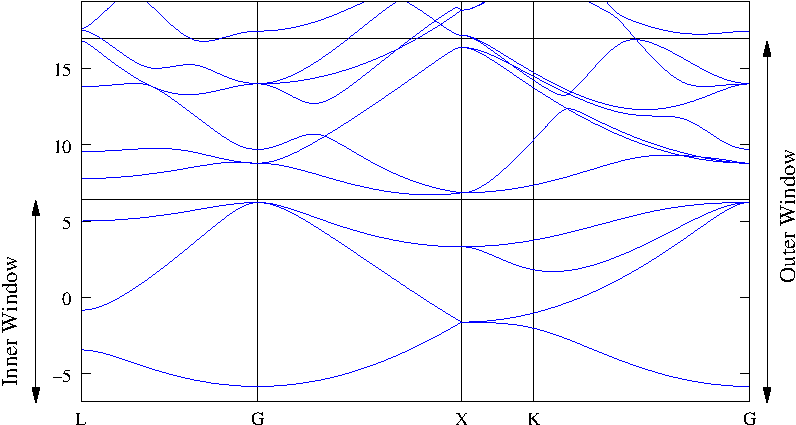
\includegraphics{si}
%\caption{Band Structure of Silicon showing the position of the outer
%and inner energy windows.}
%\label{fig:si.bnd}
%\end{center}
%\end{figure}

\cleardoublepage


\sectiontitle{17: Iron -- Spin-orbit-coupled bands and
Fermi-surface contours}

Note: It is recommended that you go through Example 8 first (bcc Fe
without spin-orbit).

\begin{itemize}
\item{Outline: \it{Plot the spin-orbit-coupled bands of ferromagnetic
      bcc Fe.  Plot the Fermi-surface contours on a plane in the
      Brillouin zone.}}
\item{Directory: {\tt examples/example17/}}
\item{Input files}
\begin{itemize}
\item{ {\tt Fe.scf} {\it The \pwscf\ input file for ground state
    calculation}}
\item{ {\tt Fe.nscf}  {\it The \pwscf\ input file to obtain Bloch
    states on a uniform grid}} 
\item{ {\tt Fe.pw2wan}  {\it The input file for {\tt pw2wannier90}}}

\item{ {\tt Fe.win}  {\it The {\tt wannier90} and {\tt postw90} input file}}
\end{itemize}
\end{itemize}

Note that {\tt num\_wann =18} in {\tt Fe.win}, but only nine trial
orbitals are provided. The line
  {\tt
\begin{quote}
spinors = true
\end{quote}
}tells {\tt wannier90} to use in step~3 below the specified trial
orbitals on both the up- and down-spin channels, effectively doubling
their number.

\begin{enumerate}
\item Run \pwscf\ to obtain the ferromagnetic ground state of
  iron\footnote{Please note the following counterintiutive feature in
    {\tt pwscf}: in order to obtain a ground state with magnetization
    along the {\it positive} $z$-axis, one should use a {\it negative}
    value for the variable {\tt starting\_magnetization}.}\\
  {\tt pw.x < Fe.scf > scf.out}

\item Run \pwscf\ to obtain the Bloch states on a uniform k-point
  grid\\ 
{\tt pw.x < Fe.nscf > nscf.out}

\item Run \wannier\ to generate a list of the required overlaps (written
  into the {\tt Fe.nnkp} file)\\
{\tt wannier90.x -pp Fe}

\item Run {\tt pw2wannier90} to compute:
  \begin{itemize}

  \item[{\bf --}] The overlaps $\langle u_{n{\bf k}}\vert u_{m{\bf
        k}+{\bf b}}\rangle$ between {\it spinor} Bloch states (written
    in the {\tt Fe.mmn} file)

  \item[{\bf --}] The projections for the starting guess (written in
    the {\tt Fe.amn} file)

  \item[{\bf --}] The spin matrix elements $\langle \psi_{n{\bf
        k}}\vert \sigma_i\vert \psi_{m{\bf k}}\rangle$, $i=x,y,z$
    (written in the {\tt Fe.spn} file)
%\item{The matrix elements  $\langle u_{n{\bf k}+{\bf b}_1}\vert H_{\bf k}\vert
%u_{m{\bf k}+{\bf
%          b}_2}\rangle$ (written in the {\tt
%        Fe.uHu} file)}
  \end{itemize}
{\tt pw2wannier90.x < Fe.pw2wan > pw2wan.out}

\item Run \wannier\ to compute the MLWFs.\\
{\tt wannier90.x Fe}

\item Run \postw\ to compute the energy eigenvalues and spin
  expectation values.\\
  {\tt postw90.x Fe} (serial execution) 

  Note: the routines for {\tt kpath=true} and {\tt kslice=true} are
  currently not parallelized over $k$-points.\\

\end{enumerate}

 In this example we use the module {\tt kpath} to plot the energy
  bands coloured by the expectation value of the spin along [001]:
  {\tt
\begin{quote}
kpath = true

kpath\_task = bands

kpath\_bands\_colour = spin     

kpath\_num\_points=500
\end{quote} }


To plot the bands using {\tt gnuplot} (version 4.2 or higher) issue
%
{\tt
\begin{quote}
myshell> gnuplot

gnuplot> load `Fe-bands.gnu'
\end{quote} }
%
or, using {\tt python},
%
{\tt
\begin{quote}
myshell> python Fe-bands.py
\end{quote} }

Next we plot the Fermi-surface contours on the (010) plane, using the
{\tt kslice} module. Set {\tt kpath = false} and uncomment the following instructions in {\tt
  Fe.win}, {\tt
\begin{quote}
kslice = true

kslice\_task = fermi\_lines

kslice\_fermi\_level = 12.6285

kslice\_corner = 0.0  0.0  0.0

kslice\_b1 =     0.5 -0.5 -0.5

kslice\_b2 =     0.5  0.5  0.5

kslice\_2dkmesh = 200 200
\end{quote} }

The Fermi level is taken from {\tt scf.out}, and the energy
eigenvalues are computed on a $200\times 200$ $k$-point grid covering
the BZ slice. The lines of intersection between the Fermi surface and
the (010) plane can be visualized with the {\tt gnuplot} or {\tt
  python} scripts generated at runtime,
%
{\tt
\begin{quote}
myshell> gnuplot

gnuplot> load `Fe-kslice-fermi\_lines.gnu'
\end{quote} }
%
%(do not be concerned by the warning messages, they are caused by the
%fact that not all bands cross the Fermi energy) 
or 
%
{\tt
\begin{quote}
myshell> python Fe-kslice-fermi\_lines.py
\end{quote} }
%
The Fermi lines can be colour-coded by the spin expectation value
$\langle S_z\rangle$ of the states on the Fermi surface. Add to {\tt
  Fe.win} the line {\tt
\begin{quote}
kslice\_fermi\_lines\_colour = spin
\end{quote} }
%
and re-run {\tt postw90}. The names of the {\tt gnuplot} and {\tt
  python} scripts generated at runtime are unchanged. (However, the
plotting algorithm is different in this case, and the lines are not as
smooth as before. You may want to increase {\tt kslice\_2dkmesh}.)

In Example~8 we obtained MLWFs separately for the up- and down-spin
channels of bcc Fe without spin-orbit. The Wannier-interpolated DOS
was therefore automatically separated into minority and majority
contributions.  For a spinor calculation we can still spin-decompose
the DOS, using
%
{\tt
\begin{quote}
dos = true

spin\_decomp = true

dos\_kmesh = 25 25 25
\end{quote} }
%
The data file {\tt Fe-dos.dat} created by {\tt postw90} contains the
up-spin and down-spin contributions in the third and fourth columns,
%
{\tt
\begin{quote}
myshell> gnuplot

gnuplot> plot 'Fe-dos.dat' u (-\$3):(\$1-12.6285) w l,'Fe-dos.dat' u (\$4):(\$1-12.6285) w l
\end{quote} }
%
An alternative approach is to project the DOS onto the up-spin and
down-spin WFs separately. To find the DOS projected onto the up-spin
(odd-numbered) WFs replace {\tt spin\_decomp = true} with
%
{\tt
\begin{quote}
  dos\_project = 1,3,5,7,9,11,13,15,17
\end{quote} }
%
and re-run {\tt postw90}. This approach has the advantage that it does
not require the {\tt Fe.spn} file.

%\subsection*{Further ideas}

%\begin{itemize}

%\item Plot the energy bands over a single line segment in $k$-space,
%  e.g., $\Gamma$--H, to see in detail a spin-orbit-induced avoided
%  crossing between majority and minority bands. [Hint: When using {\tt
%    gnuplot} you can zoom in by right-clicking to select a region of
%  the plot.]

%\item Generate the Fermi-surface contours on the (001) plane
%perpendicular to the magnetization. Note the higher symmetry compared
%to the (010) plane.

%\item Redraw the Fermi-surface contours starting from an {\it ab
%    initio} calculation without spin-orbit coupling (as in Example~8),
%  and note the changes in their connectivity.

%\end{itemize}

\cleardoublepage

\sectiontitle{18: Iron -- Berry curvature, anomalous Hall
  conductivity and optical conductivity}

\begin{itemize}
\item{Outline: \it{Calculate the Berry curvature, anomalous Hall
      conductivity, and (magneto)optical conductivity of ferromagnetic
      bcc Fe with spin-orbit coupling. In preparation for this example
      it may be useful to read Ref.~\cite{yao-prl04} and Ch.~11 of the
      User Guide.}}
\item{Directory: {\tt examples/example18/}}
\item{Input files}
\begin{itemize}
\item{ {\tt Fe.scf} {\it The \pwscf\ input file for ground state
    calculation}}
\item{ {\tt Fe.nscf}  {\it The \pwscf\ input file to obtain Bloch
    states on a uniform grid}} 
\item{ {\tt Fe.pw2wan}  {\it The input file for {\tt pw2wannier90}}}
\item{ {\tt Fe.win}  {\it The {\tt wannier90} and {\tt postw90} input file}}
\end{itemize}
\end{itemize}

The sequence of steps below is the same of Example~17.  If you have
already run that example, you can reuse the output files from steps
1--5, and only step 6 must be carried out again using the new input
file {\tt Fe.win}.

\begin{enumerate}
\item Run \pwscf\ to obtain the ground state of iron\\
{\tt pw.x < Fe.scf > scf.out}

\item Run \pwscf\ to obtain the Bloch states on a uniform k-point
  grid\\ 
{\tt pw.x < Fe.nscf > nscf.out}

\item Run \wannier\ to generate a list of the required overlaps (written
  into the {\tt Fe.nnkp} file)\\
{\tt wannier90.x -pp Fe}

\item Run {\tt pw2wannier90} to compute the overlaps between Bloch
  states and the projections for the starting guess (written in the
  {\tt Si.mmn} and {\tt  Si.amn} files)\\
{\tt pw2wannier90.x < Fe.pw2wan > pw2wan.out}

\item Run \wannier\ to compute the MLWFs\\
{\tt wannier90.x Fe}

\item Run \postw\ \\
  {\tt postw90.x Fe} (serial execution)\\
  {\tt mpirun -np 8 postw90.x Fe} (example of parallel execution with 8 nodes) 

\end{enumerate}

\subsection*{Berry curvature plots}

The Berry curvature $\Omega_{\alpha\beta}({\bf k})$ of the occupied
states is defined in Eq.~(11.18) of the User Guide.  The following
lines in {\tt Fe.win} are used to calculate the energy bands and the
Berry curvature (in bohr$^2$) along high-symmetry lines in $k$-space.
{\tt
\begin{quote}
fermi\_energy = 12.6285

berry\_curv\_unit = bohr2

kpath = true

kpath\_task = bands+curv

kpath\_bands\_colour = spin

kpath\_num\_points = 1000
\end{quote} }

%The path specification in {\tt Fe.win} is the same as in Example~17, and 
 

After executing {\tt postw90}, make the plot using the script
generated at runtime, {\tt
\begin{quote}
myshell> python Fe-bands+curv\_z.py
\end{quote} }

and compare with Fig.~2 of Ref.~\cite{yao-prl04}.  

In Example~17 we plotted the Fermi lines on the (010) plane.  To
combine them with a heatmap plot of (minus) the Berry curvature set
{\tt kpath = false}, uncomment the following lines in {\tt Fe.win},
\smallskip {\tt
\begin{quote}
kslice = true

kslice\_task = curv+fermi\_lines

kslice\_corner = 0.0  0.0  0.0

kslice\_b1 =     0.5 -0.5 -0.5

kslice\_b2 =     0.5  0.5  0.5

kslice\_2dkmesh = 200 200
\end{quote} }
%
re-run {\tt postw90}, and issue
%
{\tt
\begin{quote}
myshell> python Fe-kslice-curv\_z+fermi\_lines.py
\end{quote} }
\medskip
%
Compare with Fig.~3 in Ref.~\cite{yao-prl04}.

\subsection*{Anomalous Hall conductivity}

The intrinsic anomalous Hall conductivity (AHC) is proportional to the
BZ integral of the Berry curvature. To evaluate the AHC using a
$25\times 25\times 25$ $k$-point mesh, set {\tt kslice = false},
uncomment the following lines in {\tt Fe.win}, {\tt
\begin{quote}
berry = true

berry\_task = ahc                

berry\_kmesh = 25 25 25

\end{quote} } and re-run {\tt postw90}.  The AHC is written in the output file
{\tt Fe.wpout}.
%The $x$, $y$, and $z$ components correspond to $\sigma^{\rm
%  AH}_{yz}$, $\sigma^{\rm AH}_{zx}$, and $\sigma^{\rm AH}_{xy}$
%respectively. 
For bcc Fe with the magnetization along [001], only the $z$-component
is nonzero.
%(the tiny values of the other two components are numerical noise).

As a result of the strong and rapid variations of the Berry curvature
across the BZ, the AHC converges rather slowly with $k$-point
sampling, and a $25\times 25\times 25$ does not yield a well-converged
value.

  \begin{itemize}

  \item[{\bf --}] Increase the BZ mesh density by changing {\tt
      berry\_kmesh}.

  \item[{\bf --}] To accelerate the convergence, adaptively refine the
    mesh around spikes in the Berry curvature, by adding to {\tt
      Fe.win} the lines \smallskip {\tt
      \begin{quote}
        berry\_adpt\_kmesh = 5  
        
        berry\_adpt\_kmesh\_thresh = 100.0
      \end{quote} }

  \end{itemize}
    
    This adds a $5\times 5\times 5$ fine mesh around those points
    where $\vert\Omega_z({\bf k})\vert$ exceeds 100~bohr$^2$. The
    percentage of points triggering adaptive refinement is reported in
    {\tt Fe.wpout}.

    Compare the converged AHC value with those obtained in
    Refs.~\cite{wang-prb06} and~\cite{yao-prl04}.

    The Wannier-interpolation formula for the Berry curvature
    comprises three terms, denoted $D$-$D$, $D$-$\overline{A}$, and
    $\overline{\Omega}$ in Ref.~\cite{wang-prb06}, and $J2$, $J1$, and
    $J0$ in Ref.~\cite{lopez-prb12}.  To report in {\tt Fe.wpout} the
    decomposition of the AHC into these three terms, set {\tt iprint}
    (verbosity level) to a value larger than one in {\tt Fe.win}.

\subsection*{Optical conductivity}

The optical conductivity tensor of bcc Fe with magnetization along
$\hat{\bf z}$ has the form
%
$$
\bm{\sigma}=\bm{\sigma}^{\rm S}+\bm{\sigma}^{\rm A}=
\left(
\begin{array}{ccc}
\sigma_{xx} & 0 & 0\\
0 & \sigma_{xx} & 0\\
0 & 0 & \sigma_{zz}
\end{array}
\right)+
\left(
\begin{array}{ccc}
0 & \sigma_{xy} & 0 \\
-\sigma_{xy} & 0 & 0\\
0 & 0 & 0
\end{array}
\right)$$
%
where ``S'' and ``A'' stand for the symmetric and antisymmetric parts
and $\sigma_{xx}=\sigma_{yy}\not=\sigma_{zz}$. The dc AHC calculated
earlier corresponds to $\sigma_{xy}$ in the limit $\omega\rightarrow
0$. At finite frequency $\sigma_{xy}$ acquires an imaginary part which
describes magnetic circular dichoism (MCD).

To compute the complex optical conductivy for $\hbar\omega$
up to 7~eV, replace 
{\tt
\begin{quote}
berry\_task = ahc
\end{quote} }
%
with
%
{\tt
\begin{quote}
berry\_task = kubo
\end{quote} }
%
add the line
%
{\tt
\begin{quote}
kubo\_freq\_max = 7.0
\end{quote} }
%
and re-run {\tt postw90}. Reasonably converged spectra can be
obtained with a $125\times 125\times 125$ $k$-point mesh. Let us first
plot the ac AHC in S/cm, as in the lower panel of Fig.~5 in
Ref.~\cite{yao-prl04}, {\tt
\begin{quote}
myshell> gnuplot

gnuplot> plot `Fe-kubo-A\_xy.dat' u 1:2 w l
\end{quote} }

Comapare the $\omega\rightarrow 0$ limit with the result obtained
earlier by integrating the Berry curvature.\footnote{The calculation
  of the AHC using {\tt berry\_task = kubo} involves a truncation of
  the sum over empty states in the Kubo-Greenwood formula: see
  description of the keyword {\tt kubo\_eigval\_max} in the User
  Guide. As discussed around Eq.~(11.17) of the User Guide, no
  truncation is done with {\tt berry\_task = ahc}.}


Next we plot the MCD spectrum. Following Ref.~\cite{yao-prl04}, we
plot ${\rm Im}[\omega\sigma_{xy}(\hbar\omega)]$, in units of
$10^{29}$~sec$^{-2}$. The needed conversion factor is $9\times
10^{-18}\times e/\hbar\simeq 0.0137$ ($e$ and $\hbar$ in SI units),
{\tt
\begin{quote}
gnuplot> set yrange[-5:15]

gnuplot> plot `Fe-kubo-A\_xy.dat' u 1:(\$1)*(\$3)*0.0137 w l
\end{quote} }

\subsection*{Further ideas}

\begin{itemize}

\item Recompute the AHC and optical spectra of bcc Fe using projected
  $s$, $p$, and $d$-type Wannier functions instead of the hybridrized
  MLWFs (see Example~8), and compare the results.

\item Redraw the Fermi surface contours on the (010) plane starting
  from a calculation without spin-orbit coupling, by adding to the
  input files {\tt iron\_\{up,down\}.win} in Example~8 the lines
{\tt
\begin{quote}
kslice = true

kslice\_task = fermi\_lines

kslice\_fermi\_level = 12.6256

kslice\_corner = 0.0  0.0  0.0

kslice\_b1 =     0.5 -0.5 -0.5

kslice\_b2 =     0.5  0.5  0.5

kslice\_2dkmesh = 200 200
\end{quote} }
%
before running {\tt postw90},
%
{\tt
\begin{quote}
postw90.x iron\_up

postw90.x iron\_dn
\end{quote}
}
%
The {\tt python} scripts generated at runtime draw the up- and
down-spin Fermi lines on separate figures. To draw them together, use
the script {\tt iron\_updn-kslice-fermi\_lines.py} provided with
Example~18 (or merge the two generated scripts). Compare the Fermi
lines with and without spin-orbit; look back at the Berry curvature
heatmap plot, and note how the ``hot-spots'' tend to occur near
spin-orbit-induced avoided crossings.

\item A crude way to model the influence of heterovalent alloying on
  the AHC is to assume that its only effect is to donate or deplete
  electrons, i.e., to shift the Fermi level of the pure
  crystal~\cite{yao-prb07}.

Recalculate the AHC of bcc Fe for a range of Fermi energies within
$\pm 0.5$~eV of the true Fermi level. This calculation can be
streamlined by replacing in {\tt Fe.win} {\tt
\begin{quote}
fermi\_energy = 12.6285
\end{quote} }
%
with
%
{\tt
\begin{quote}
fermi\_energy\_min = 12.1285

fermi\_energy\_max = 13.1285
\end{quote} }
%
Use a sufficiently dense BZ mesh with adaptive refinement. To plot
$\sigma_{xy}$ versus $\varepsilon_F$, issue
%
{\tt
\begin{quote}
myshell> gnuplot

gnuplot> plot `Fe-ahc-fermiscan.dat' u 1:4 w lp
\end{quote} }

\end{itemize}


\cleardoublepage

\sectiontitle{19: Iron -- Orbital magnetization}


\begin{itemize}
\item{Outline: \it{Calculate the orbital magnetization of
      ferromagnetic bcc Fe by Wannier interpolation.}}
\item{Directory: {\tt examples/example19/}}
\item{Input files}
\begin{itemize}
\item{ {\tt Fe.scf} {\it The \pwscf\ input file for ground state
    calculation}}
\item{ {\tt Fe.nscf}  {\it The \pwscf\ input file to obtain Bloch
    states on a uniform grid}} 
\item{ {\tt Fe.pw2wan}  {\it The input file for {\tt pw2wannier90}}}
\item{ {\tt Fe.win} {\it The {\tt wannier90} and {\tt postw90} input
      file}}
\end{itemize}
\end{itemize}

The sequence of steps below is the same of Examples~17 and 18.  If you
have already run one of those examples, you can reuse the output files
from steps 1--3 and 5. Steps~4 and 6 should be carried out again using
the new input files {\tt Fe.pw2wan} and {\tt Fe.win}.

\begin{enumerate}
\item Run \pwscf\ to obtain the ground state of iron\\
{\tt pw.x < Fe.scf > scf.out}

\item Run \pwscf\ to obtain the Bloch states on a uniform k-point
  grid\\ 
{\tt pw.x < Fe.nscf > nscf.out}

\item Run \wannier\ to generate a list of the required overlaps (written
  into the {\tt Fe.nnkp} file).\\
{\tt wannier90.x -pp Fe}


\item Run {\tt pw2wannier90} to compute:
  \begin{itemize}

  \item[{\bf --}] The overlaps $\langle u_{n{\bf k}}\vert u_{m{\bf k}+{\bf
          b}}\rangle$ (written in the {\tt Fe.mmn} file)

  \item[{\bf --}] The projections for the starting guess (written in the {\tt
        Fe.amn} file)

  \item[{\bf --}] The matrix elements $\langle u_{n{\bf k}+{\bf b}_1}\vert
      H_{\bf k}\vert u_{m{\bf k}+{\bf b}_2}\rangle$ (written in the
      {\tt Fe.uHu} file)

%  \item[{\bf --}] The spin matrix elements $\langle \psi_{n{\bf
%        k}}\vert \sigma_i\vert \psi_{m{\bf k}}\rangle$ (written in the
%    {\tt Fe.spn} file)

  \end{itemize}
{\tt pw2wannier90.x < Fe.pw2wan > pw2wan.out}

\item Run \wannier\ to compute the MLWFs.\\
{\tt wannier90.x Fe}

\item Run \postw\ to compute the orbital magnetization.\\
  {\tt postw90.x Fe} (serial execution)\\
  {\tt mpirun -np 8 postw90.x Fe} (example of parallel execution with 8 nodes) 


\end{enumerate}

The orbital magnetization is computed as the BZ integral of the
quantity ${\bf M}^{\rm orb}({\bf k})$ defined in Eq.~(11.20) of the
User Guide. The relevant lines in {\tt Fe.win} are
%
{\tt
\begin{quote}
berry = true

berry\_task = morb

berry\_kmesh = 25 25 25

fermi\_energy = 12.6285
\end{quote} }
%
After running {\tt postw90}, compare the value of the orbital
magnetization reported in {\tt Fe.wpout} with the spin magnetization
in {\tt scf.out}. Set {\tt iprint = 2} to report the decomposition of
${\bf M}^{\rm orb}$ into the terms $J0$, $J1$, and $J2$ defined in
Ref.~\cite{lopez-prb12}.
%\footnote{Alternatively, the
%spin magnetization can be computed by {\tt postw90}. This requires adding the
%instruction {\tt spin\_moment = T} to {\tt Fe.win}, assuming that {\tt pw2wannier90}
%was executed with {\tt write\_spn = .true.} in {\tt Fe.pw2wan}.} 
%Both point along $\hat{\bf
%  z}$, but the orbital contribution is much smaller (it is strongly
%quenched by the crystal field).

To plot $M_z^{\rm orb}({\bf k})$ along high-symmetry lines set {\tt
  berry = false} and uncomment in {\tt Fe.win} the block of
instructions containing {\tt
\begin{quote}
kpath = true

kpath\_task = bands+morb
\end{quote}
}
After running {\tt postw90}, issue
%
{\tt
\begin{quote}
myshell> python Fe-bands+morb\_z.py
\end{quote} } 
%
Compare with Fig.~2 of Ref.~\cite{lopez-prb12}, bearing in mind the
factor of $-1/2$ difference in the definition of ${\bf M}^{\rm
  orb}({\bf k})$ (see Ch.~11 in the User Guide).

To plot $M_z^{\rm orb}({\bf k})$ together with the Fermi contours on the
(010) BZ plane set {\tt kpath = false}, uncomment in {\tt
  Fe.win} the block of instructions containing 
{\tt
\begin{quote}
kslice = true

kslice\_task = morb+fermi\_lines
\end{quote}
} 
re-run {\tt postw90}, and issue
{\tt
\begin{quote}
myshell> python Fe-kslice-morb\_z+fermi\_lines.py
\end{quote} }
%
$M_z^{\rm orb}({\bf k})$ is much more evenly distributed in $k$-space
than the Berry curvature (see Example 18). As a result, the integrated
orbital magnetization converges more rapidly with the BZ sampling.


\cleardoublepage

\bibliographystyle{apsrev4-1}
\bibliography{../wannier90}

\end{document}
